\documentclass{article}

\usepackage{graphicx}
\usepackage{caption}
\usepackage{subcaption}
\usepackage{listings}

\begin{document}
\begin{titlepage}
	\begin{center}
		
\includegraphics[width=0.5\textwidth]{assets/ku.png}\\[1cm]
		\textsc{\LARGE Kathmandu University}\\[0.2cm]
		\textsc{\large department of computer science and engineering}\\[2cm]

\textsc{\Large Database management system}\\[0.2cm]
\textsc{\large COMP232}\\[1cm]

\hrule \vspace{0.5cm}
{\Large Lab 2 Report} \\[0.5cm]
\hrule \vspace{0.5cm}


\large
\emph{Author:}\\
Ashish Thapa (56)\\[1cm]


\emph{Submitted To:}\\
Rajani Chulaydyo \\[1.5cm]

% Author info
{\large \today}\\[1cm]

\end{center}
\end{titlepage}

\tableofcontents

\section{Schema For DDL}
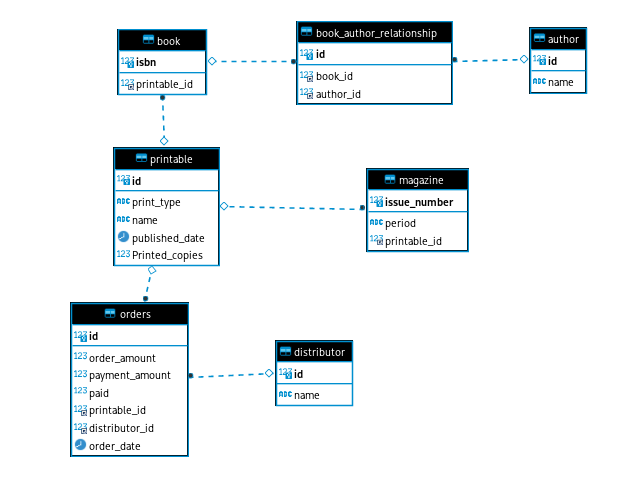
\includegraphics{assets/erd.png}

\section{DDL Script for creating tables and populating it}

\begin{lstlisting}
CREATE TABLE author(
id INT PRIMARY KEY,
name VARCHAR(255)
);

INSERT INTO author(id,name) VALUES
(1,"Rumi"),
(2,"Malcom Gladwell"),
(3,"Victor Frankl"),
(4,"Johan Abildskov");


CREATE TABLE IF NOT EXISTS printable (                                     
id INT PRIMARY KEY,                                                        
print_type VARCHAR(255),                                                   
name VARCHAR (255),                                                        
published_date DATE,                                                       
Printed_copies INT                                                       
);

INSERT INTO printable(id,print_type,name,published_date,printed_copies) VALUES
(1, "book", "A Masnavi", "1992-12-01",1234547),
(2, "book", "A Strangers", "2003-12-01",1245),
(3, "book", "Man Search for Meaning", "2018-12-01",823),
(4, "magazine", "A GCT", "1992-12-01",1234547),
(5, "magazine", "Nature", "2023-01-01",1234547),
(6, "book", "Practical Git", "2013-02-12",1234547);

INSERT INTO printable(id,print_type,name,published_date,printed_copies) VALUES
(7, "book", "Practical Git For Quantum Computers", "2023-02-12",1234547);

CREATE TABLE IF NOT EXISTS book (                                          
isbn INT PRIMARY KEY,    
printable_id INT,
FOREIGN KEY(printable_id) REFERENCES printable(id)                         
);  

INSERT INTO book(isbn, printable_id) VALUES
(1,1),
(2,2),
(3,3),
(4,6);
CREATE TABLE IF NOT EXISTS magazine (                                      
issue_number INT PRIMARY KEY,                                              
period VARCHAR(40),
printable_id INT,
FOREIGN KEY(printable_id) REFERENCES printable(id)                         
);

INSERT INTO magazine(issue_number,period, printable_id) VALUES 
(1,"monthly",4),
(2,"weekly",5);

CREATE TABLE IF NOT EXISTS book_author_relationship (
id SERIAL PRIMARY KEY,
book_id INT,
author_id INT,
FOREIGN KEY(book_id) REFERENCES book(isbn),                                
FOREIGN KEY(author_id) REFERENCES author(id)                           
);

INSERT INTO book_author_relationship (id, book_id, author_id) VALUES 
(1,1,1),
(2,2,2),
(3,3,3),
(4,4,4);

CREATE TABLE IF NOT EXISTS distributor (                                   
id INT PRIMARY KEY,                                                        
name VARCHAR(255)                                                     
); 

INSERT INTO distributor (id, name) VALUES 
(1,"Heritage Publication"),
(2,"Starch Press");

CREATE TABLE IF NOT EXISTS orders (                                        
id INT PRIMARY KEY,                                                        
order_amount INT,                                                          
payment_amount INT,                                                        
paid BOOL,
printable_id INT,
distributor_id INT,
order_date DATE,
FOREIGN KEY(printable_id) REFERENCES printable(id) ON DELETE CASCADE,      
FOREIGN KEY(distributor_id) REFERENCES distributor(id) ON DELETE CASCADE
);

INSERT INTO orders (id, order_amount, payment_amount, paid, printable_id, distributor_id,order_date) VALUES 
(1,763,900000,false,1,1,'2013-02-12'),
(6,89002,434534532,true,6,2,'2022-12-10'),
(2,8900,4332,true,6,1,'2022-12-10'),
(4,8900,4332,true,6,2,'2022-12-10');	
\end{lstlisting}
\section{Queries in Relational Algebra and SQL with their output table}

\subsection{Find the name of all published books}

\begin{flushleft}
	From printable table we select all the entries that are already published and the type is book.
\end{flushleft}
\begin{lstlisting}[frame=single]
SELECT * FROM printable p WHERE p.print_type LIKE 'book'
AND p.published_date <= NOW();	
\end{lstlisting} 

\[
	\sigma_{p.print\_type\ LIKE\ 'book'\ AND\ p.published\_date \le NOW()}(\rho_{p}(printable))
.\]

\begin{table}[h]
\begin{tabular}{lllll}
id & print\_type & name                   & published\_date & Printed\_copies \\
1  & book        & A Masnavi              & 1992-12-01      & 1234547         \\
2  & book        & A Strangers            & 2003-12-01      & 1245            \\
3  & book        & Man Search for Meaning & 2018-12-01      & 823             \\
6  & book        & Practical Git          & 2013-02-12      & 1234547        
\end{tabular}
\end{table}


\subsection{Find the name of all books published before 2000}

\begin{flushleft}
	The constraint here is published date for the entries on printable table must be less than Jan of 2001.
\end{flushleft}
\begin{lstlisting}[frame=single]
SELECT * FROM printable p 
WHERE p.published_date < '2000-01-01';
\end{lstlisting}

\[
	\sigma_{p.published\_date \le '2000-01-01'}(\rho_{p}(printable))
.\]


\begin{table}[h]
\begin{tabular}{lllll}
id & print\_type & name      & published\_date & Printed\_copies \\
1  & book        & A Masnavi & 1992-12-01      & 1234547         \\
4  & magazine    & A GCT     & 1992-12-01      & 1234547        
\end{tabular}
\end{table}


\subsection{Get the details of the books written by particular author}


Tables \textbf{printable}, \textbf{book}, \textbf{book\_author\_relationship} and \textbf{author} are joined together and then we get the name of the book by particular author if we add constraint  author.name\ LIKE\ 'author\_name' 

\[

\Pi_{p.*, a . name}
 (\rho_p(printable) \bowtie_{b.printable\_id = p.id}

\rho_b(book)\bowtie_{bar.book\_id = b.isbn}

\rho_bar(book\_author\_relationship)\bowtie_{a.id = bar.author\_id} \rho_a(author))
.\]\\[0.3cm]

\begin{lstlisting}[frame=single]
SELECT p.*, b.*  FROM printable p 
INNER JOIN book b on b.printable_id  = p.id 
INNER JOIN book_author_relationship bar 
ON bar.book_id = b.isbn 
INNER JOIN author a 
ON a.id = bar.author_id;
\end{lstlisting}

\begin{table}[h]
\begin{tabular}{llllll}
id & print\_type & name                   & published\_date & Printed\_copies & name            \\
1  & book        & A Masnavi              & 1992-12-01      & 1234547         & Rumi            \\
2  & book        & A Strangers            & 2003-12-01      & 1245            & Malcom Gladwell \\
3  & book        & Man Search for Meaning & 2018-12-01      & 823             & Victor Frankl   \\
6  & book        & Practical Git          & 2013-02-12      & 1234547         & Johan Abildskov
\end{tabular}
\end{table}


\subsection{Find the name of all weekly publications}
\[

\Pi_{p.name, m.period}
(\rho_{period LIKE "weekly"}

  (\rho_p(printable) \bowtie_{m.printable\_id = p .id} \rho_m(magazine)))

.\]

\begin{lstlisting}[frame=single]
SELECT p.*,m.* FROM printable p 
INNER JOIN magazine m 
ON m.printable_id = p.id WHERE period LIKE 'weekly';
\end{lstlisting}

\begin{table}[h]
\begin{tabular}{lllllll}
id & print\_type & name   & published\_date & Printed\_copies & issue\_number & period  \\
5  & magazine    & Nature & 2018-01-01      & 1234547         & 2             & weekly             
\end{tabular}
\end{table}


\subsection{Find the name of pre-ordered books}
\[

\Pi_{p.*, o.order\_date, o.order\_amount}(

 \sigma_{p.printed_copies < o . order\_amount AND p . print\_type LIKE "book"}

  (\rho_p(printable)\bowtie_{o.printable\_id = p.id} \rho_o{orders}))
.\]

\begin{lstlisting}[frame=single]
SELECT p.*,o.order_date,o.order_amount  FROM printable p 
INNER JOIN orders o ON o.printable_id = p.id 
WHERE p.Printed_copies < o.order_amount 
AND p.print_type like 'book';
\end{lstlisting}

\begin{table}[h]
\begin{tabular}{lllllll}
id & print\_type & name        & published\_date & Printed\_copies & order\_date & order\_amount \\
2  & book        & A Strangers & 2003-12-01      & 1245            & 2022-12-10  & 8900         
\end{tabular}
\end{table}


\subsection{Get the details of all publications with the name starting with an 'A'}

\[

	\sigma_{p.name LIKE 'a\%'}(\rho_pprintable)

.\]

\begin{lstlisting}[frame=single]
SELECT * FROM printable p WHERE p.name LIKE 'a%';
\end{lstlisting}
\begin{table}[h]
\begin{tabular}{lllll}
id & print\_type & name        & published\_date & Printed\_copies \\
1  & book        & A Masnavi   & 1992-12-01      & 1234547         \\
2  & book        & A Strangers & 2003-12-01      & 1245            \\
4  & magazine    & A GCT       & 1992-12-01      & 1234547        
\end{tabular}
\end{table}
\pagebreak
\subsection{Find all the orders for a particular book.The result must be sorted based on the order date}

\[

	
 \Pi_{p.name,p.printed\_copies,o.order\_amount, o.order\_date}(

  \sigma_{p.print\_type LIKE "book"}
   (\rho_p(printable) \bowtie_{p.id = o.printable\_id}
    \rho_oorders)

.\]

\begin{flushleft}
	
\end{flushleft}

\begin{lstlisting}[frame=single]
SELECT * from printable p 
INNER JOIN orders o ON 
p.id = o.printable_id
WHERE p.print_type LIKE 'book'
ORDER BY p.name, o.order_date;
\end{lstlisting}
\begin{table}[h]
\begin{tabular}{llll}
name          & Printed\_copies & order\_amount & order\_date \\
A Masnavi     & 1234547         & 763           & 2013-02-12  \\
A Masnavi     & 1234547         & 763           & 2013-02-12  \\
A Masnavi     & 1234547         & 763           & 2013-02-12  \\
A Strangers   & 1245            & 8900          & 2022-12-10  \\
Practical Git & 1234547         & 8900          & 2022-12-10  \\
Practical Git & 1234547         & 8900          & 2022-12-10  \\
Practical Git & 1234547         & 8900          & 2022-12-10  \\
Practical Git & 1234547         & 89002         & 2022-12-10  \\
Practical Git & 1234547         & 89002         & 2022-12-10 
\end{tabular}
\end{table}
\end{document}


